%% Eq_methods.tex
%% Simplified equations for Section 4: Methodology
%% Notation: r_k = source tokens at scale k,  A_k = cross-attention map,
%%           a_{k,b} = per-block focus attention,  \hat{a}_k = IQR-filtered attention,
%%           M_k^f = focus mask,  M_k^p = preserve mask,  M_k^rep = replacement mask,
%%           g_k = generated target tokens,  r_k = final output tokens

%% Eq. 1 — BSQ-VAE source image encoding
\newcommand{\EqBsqEncode}{%
\begin{equation}
    \{r_k^s\}_{k=1}^{S} = \mathcal{Q}_{\mathrm{BSQ}}\!\bigl(\mathcal{E}(I_{\mathrm{src}})\bigr),
    \label{eq:bsq_encode}
\end{equation}}

%% Eq. 2 — IQR fence: blocks retained after outlier removal
\newcommand{\EqIqrFilter}{%
\begin{equation}
    \mathcal{B}_{\mathrm{keep}} = \bigl\{ b \;\big|\; e_b \leq Q_3 + 1.5\,(Q_3 - Q_1) \bigr\},
    \label{eq:iqr_filter}
\end{equation}}

%% Eq. 3 — Filtered attention map (mean over retained blocks)
\newcommand{\EqFilteredAttn}{%
\begin{equation}
    \hat{a}_k = \frac{1}{|\mathcal{B}_{\mathrm{keep}}|} \sum_{b \in \mathcal{B}_{\mathrm{keep}}} a_{k,b}.
    \label{eq:filtered_attn}
\end{equation}}

%% Eq. 4a — Min-max normalization of the filtered attention map
\newcommand{\EqNormalize}{%
\begin{equation}
    \tilde{a}_k = \frac{\hat{a}_k - \min \hat{a}_k}{\max \hat{a}_k - \min \hat{a}_k}
    \;\in\; [0,1]^{N_v}.
    \label{eq:normalize}
\end{equation}}

%% Eq. 4b — CV-to-kappa mapping
\newcommand{\EqKappa}{%
\begin{equation}
    \kappa(c_k) = \kappa_{\max}\cdot
    \operatorname{clamp}\!\left(\frac{c_k - c_{\min}}{c_{\max} - c_{\min}},\,0,\,1\right),
    \qquad c_k = \frac{\sigma_k}{\mu_k},
    \label{eq:kappa}
\end{equation}}

%% Eq. 4c — Instance-adaptive threshold on the normalized map
\newcommand{\EqTau}{%
\begin{equation}
    \tau_k = h + \kappa(c_k)\cdot \tilde{\sigma}_k,
    \label{eq:tau}
\end{equation}}

%% Eq. 4d — Focus and preserve masks
\newcommand{\EqMasks}{%
\begin{equation}
\begin{aligned}
    M_k^{\mathrm{f}} &= \mathbf{1}\!\left[\tilde{a}_k \ge \tau_k\right], \\
    M_k^{\mathrm{p}} &= \mathbf{1}\!\left[\tilde{a}_k < \ell\right].
\end{aligned}
\label{eq:masks}
\end{equation}}

%% Eq. 5 — Scale-wise selective token replacement
\newcommand{\EqTokenReplace}{%
\begin{equation}
    r_k = \begin{cases}
        r_k^s & \text{if } k < N \\[2pt]
        M_k^{\mathrm{rep}} \odot r_k^s \;+\; (1{-}M_k^{\mathrm{rep}}) \odot g_k & \text{if } k \geq N
    \end{cases}
    \label{eq:token_replace}
\end{equation}}

%% --- Used in supplementary ---
%% (Coverage ratio equation removed — replaced by adaptive thresholding)

\section{Methodology}
\label{section:method}

\subsection{Overview}
\label{sec:overview}

Given a source image $I_s \in \mathbb{R}^{H \times W \times 3}$, a source prompt $P_s$, and a target prompt $P_t$, the goal of training-free image editing is to produce an edited image $I_e$ that reflects the semantic intent of $P_t$ while preserving all regions not specified by the instruction. Formally:
\begin{equation}
    I_e = f(I_s, P_s, P_t)
\end{equation}
where $f$ is realized entirely at inference time without any parameter updates.

The overall architecture of our proposed method is illustrated in Figure~\ref{fig:pipeline}. The model first resolves spatial editing semantics via cross-modal attention analysis, then selectively rewrites only the targeted tokens. Concretely, our method performs \textbf{dual-stream mask extraction} (Phases~1--2) followed by \textbf{mask-guided token composition} (Phase~3). The edited token map at each scale is:
\begin{equation}
    r_k^e = M_k^{\mathrm{rep}} \odot r_k^s + (1 - M_k^{\mathrm{rep}}) \odot g_k
\end{equation}
where $g_k$ denotes tokens generated under the target prompt, $r_k^s$ the source tokens, and $\odot$ element-wise multiplication. The final edited image $I_e$ is decoded from $\{r_k^e\}_{k=1}^{S}$ by the BSQ-VAE decoder.

\subsection{IQR-Filtered Attention Aggregation}
\label{sec:mask_construction}
\begin{figure}[t]
    \centering
    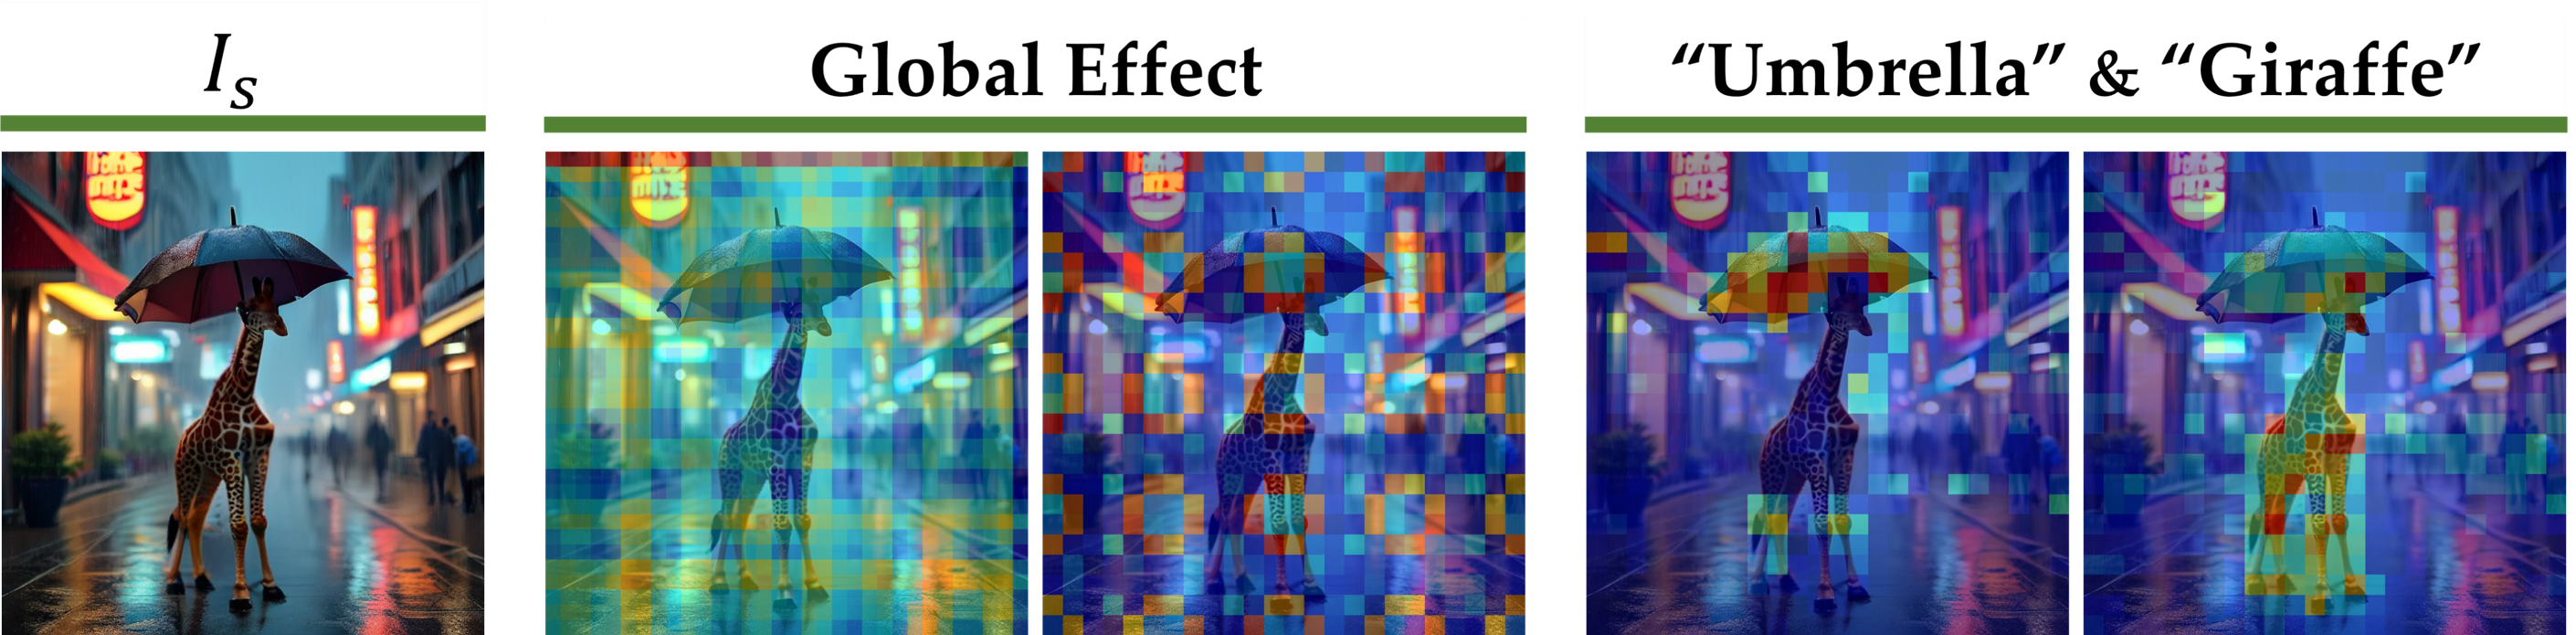
\includegraphics[width=\linewidth]{imgs/globalEffect.png}
    \caption{Global layer effect. \textbf{Middle}: blocks with positional bias produce uniform, non-localizable attention. \textbf{Right}: after IQR filtering, attention correctly focuses on ``Umbrella'' and ``Giraffe''.}
    \label{fig:globalEffect}
\end{figure}

Directly using raw cross-attention maps yields noisy and unreliable masks, because certain transformer blocks produce attention dominated by positional bias rather than semantic content --- a \textit{global layer effect} that spreads attention uniformly regardless of the text query (see Fig.~\ref{fig:globalEffect}).

We suppress these outlier transformer blocks using Interquartile Range (IQR) filtering, a non-parametric method requiring no learned parameters. Let $A_{k,b} \in \mathbb{R}^{N_v \times N_t}$ denote the cross-attention matrix at scale $k$ and transformer block $b$, where $N_v$ is the number of visual tokens and $N_t$ the number of text tokens. Let $\mathcal{F} \subset \{1, \ldots, N_t\}$ denote the set of token indices corresponding to the editing-relevant words in the prompt (e.g., ``water bottle''), identified by differencing the source and target prompts. For each transformer block $b$, we extract the columns of $A_{k,b}$ indexed by $\mathcal{F}$ and average them to obtain a spatial attention map $a_{k,b} \in \mathbb{R}^{N_v}$, which indicates how strongly each visual token attends to the focus words. We then compute the mean attention map across all blocks, $\bar{a}_k = \frac{1}{B}\sum_{b} a_{k,b}$, and measure each block's deviation as $e_b = \mathrm{MSE}(a_{k,b},\, \bar{a}_k)$. Blocks whose deviation exceeds the IQR fence are discarded:
\EqIqrFilter
where $Q_1$ and $Q_3$ are the first and third quartiles of $\{e_b\}$. The retained set $\mathcal{B}_{\mathrm{keep}}$ contains only transformer blocks whose attention maps reflect semantic content rather than positional bias. The filtered attention map is then computed as the mean over the attention maps of these retained blocks:
\EqFilteredAttn
In practice, approximately 10--20\% of blocks are filtered per scale, yielding substantially more spatially coherent attention maps.

\subsection{Instance-Adaptive Mask Binarization}
\label{sec:threshold}

The filtered map $\hat{a}_k$ must be binarized into a focus mask (regions the edit may rewrite) and a preserve mask (background used to anchor source content). This subsection derives the binarization rule, which is the component that most directly controls the preservation--edit trade-off.

\noindent\textbf{Why rank-based thresholds are structurally inadequate.}
A natural first choice is a rank-based rule: take the $p$-th percentile of $\hat{a}_k$ as the threshold. Such a rule, however, \textit{always} selects the top $(1-p)$ fraction of spatial positions, even when the map contains no salient high-energy region at all. This is not a tuning issue but a structural one: for edits such as object addition or global style transfer, the source prompt has no corresponding focus region in the source image, and the correct focus mask may legitimately be empty or near-empty. A rank-based rule cannot express this.

\noindent\textbf{What the attention statistics actually encode.}
A second natural choice is a moment-based threshold $\tau_k = \mu_k + \kappa \sigma_k$, where $\mu_k, \sigma_k$ are the mean and standard deviation of $\hat{a}_k$ and $\kappa$ is modulated by the coefficient of variation $c_k = \sigma_k / \mu_k$ so that concentrated attention yields a tighter mask. Measuring these statistics over the full benchmark, however, reveals that the between-task variation of $c_k$ is driven almost entirely by the \emph{denominator}: across ten editing categories the median $\sigma_k$ spans less than a factor of two, whereas the median $\mu_k$ spans more than a factor of three, in the direction opposite to $c_k$ (Sec.~\ref{sec:cv_analysis}). In other words, $c_k$ is effectively a measure of \textit{how large a fraction of the image the focus region occupies}, and $\mu_k$ --- not the distribution shape --- dominates the absolute scale of $\mu_k + \kappa \sigma_k$. This produces exactly the wrong behaviour in the case that matters most: when the focus word corresponds to a small, well-localized object, attention concentrates on a few positions and the remaining background drags $\mu_k$ down, so $\tau_k$ falls and the resulting mask becomes \emph{larger}.

\noindent\textbf{Absolute-energy threshold with a CV-adaptive correction.}
We therefore decouple the threshold from $\mu_k$ by min-max normalizing the filtered map,
\EqNormalize
and thresholding this normalized energy at an absolute level. The level consists of a fixed base $h$ plus an instance-adaptive correction driven by the coefficient of variation,
\EqKappa
\EqTau
where $\tilde{\sigma}_k$ is the standard deviation of the normalized map $\tilde{a}_k$, and $c_{\min}, c_{\max}, \kappa_{\max}$ define the mapping. The two masks are then
\EqMasks
where $\ell$ is the preserve level. Algorithm~\ref{alg:adaptive_threshold} summarizes the procedure.

\begin{algorithm}[t]
\caption{Instance-Adaptive Mask Binarization}
\label{alg:adaptive_threshold}
\small
\begin{algorithmic}[1]
\Require Filtered attention $\hat{a}_k \in \mathbb{R}^{N_v}$; base level $h$;
         CV range $[c_{\min}, c_{\max}]$; gain $\kappa_{\max}$; preserve level $\ell$
\Ensure Focus mask $M_k^{\mathrm{f}}$, preserve mask $M_k^{\mathrm{p}}$

\State $\mu_k \gets \mathrm{mean}(\hat{a}_k)$,\quad $\sigma_k \gets \mathrm{std}(\hat{a}_k)$
\State $c_k \gets \sigma_k / \mu_k$ \Comment{coefficient of variation, on the \emph{raw} map}
\State $\tilde{a}_k \gets \bigl(\hat{a}_k - \min \hat{a}_k\bigr) / \bigl(\max \hat{a}_k - \min \hat{a}_k\bigr)$
       \Comment{min--max normalization}
\State $\tilde{\sigma}_k \gets \mathrm{std}(\tilde{a}_k)$
\State $\kappa \gets \kappa_{\max}\cdot\operatorname{clamp}\!\bigl((c_k - c_{\min})/(c_{\max} - c_{\min}),\,0,\,1\bigr)$
\State $\tau_k \gets h + \kappa \cdot \tilde{\sigma}_k$ \Comment{$\tau_k \ge h$ since $\kappa \ge 0$}
\State $M_k^{\mathrm{f}} \gets \mathbb{1}[\tilde{a}_k \ge \tau_k]$,\quad
       $M_k^{\mathrm{p}} \gets \mathbb{1}[\tilde{a}_k < \ell]$
\State \Return $M_k^{\mathrm{f}},\, M_k^{\mathrm{p}}$
\end{algorithmic}
\end{algorithm}


Three properties of this formulation are worth making explicit.

\textit{(i) $h$ remains the single semantically meaningful knob.} We fix $\kappa_{\min} = 0$ by construction, so $\tau_k \ge h$ always holds: the adaptive term can only \emph{tighten} the mask relative to the base level, never loosen it. Sweeping $h$ traces a smooth, monotone preservation--edit frontier (Sec.~\ref{sec:frontier}), and the adaptive term shifts that frontier outward rather than adding a second, competing degree of freedom.

\textit{(ii) The focus mask can be empty.} Because the criterion is an absolute energy level rather than a rank, an attention map with no region above $\tau_k$ produces no focus mask, and the corresponding scale is left entirely to source tokens. This is the behaviour a rank-based rule cannot express.

\textit{(iii) The preserve level $\ell$ is not a tuned hyperparameter.} The preserve mask is consumed only by Phase~2, where it anchors background positions to source tokens while the target-side attention is recorded; the tokens generated in that pass are discarded (Sec.~\ref{sec:pipeline}). Consequently $\ell$ influences the final output only through whether the target attention peaks cross $\tau_k$, which it does not affect. We set $\ell = h - 0.01$ throughout.

The parameters $(h, c_{\max}, \kappa_{\max})$ are not hand-tuned; Sec.~\ref{sec:protocol} describes the four-stage protocol used to derive them and reports their sensitivity.
% TODO(verify): confirm against the CLI log of the result directory behind Table I.
% Values used in this paper: h = 0.50, c_min = 0, c_max = 0.20, kappa_min = 0, kappa_max = 0.60.

\subsection{Three-Phase Editing Pipeline}
\label{sec:pipeline}

At each generation scale, the editing pipeline executes three phases in sequence. Phase~1 injects source tokens and extracts source-side masks from cross-attention (see Fig.~\ref{fig:pipeline}), Phase~2 extracts target-side masks with background anchoring, and Phase~3 composes the final tokens by merging the two streams.

\noindent\textbf{Phase~1: Source-Stream Mask Extraction.}
To identify which spatial regions correspond to the source semantics, we generate visual tokens at scale $k$ conditioned on the source prompt $P_s$, with the continuous source features injected at every scale so that the pass reconstructs $I_s$. From the resulting cross-attention, we apply IQR filtering and thresholding (Sec.~\ref{sec:mask_construction}--\ref{sec:threshold}) to obtain the source focus mask $M_{k,s}^{\mathrm{f}}$ and the preserve mask $M_{k,s}^{\mathrm{p}}$.

\noindent\textbf{Phase~2: Target-Stream Mask Extraction.}
Composition needs to know which regions the edit will affect before any token is replaced. Since the source-side mask alone cannot capture regions newly introduced by the target prompt, we perform a second generation pass conditioned on the target prompt $P_t$, anchoring positions where $M_{k,s}^{\mathrm{p}} = 1$ to source tokens $r_k^s$ to prevent background drift. From the resulting cross-attention, we extract the target focus mask $M_{k,t}^{\mathrm{f}}$ via the same filtering and thresholding procedure. The image generated in this pass is discarded; the mask is its only output.

\noindent\textbf{Phase~3: Mask-Guided Token Composition.}
Given the dual-stream masks, we compute the replacement mask $M_k^{\mathrm{rep}} = \neg(M_{k,s}^{\mathrm{f}} \cup M_{k,t}^{\mathrm{f}})$, which marks background positions for source token substitution. We generate the target tokens $g_k$ freely under $P_t$, then assemble the final output:
\EqTokenReplace
Substitution operates on the bitwise token index $r_k \in \{0,1\}^{h_k \times w_k \times d}$, so composition is exact at the bit level and the replaced positions decode to the source content without residual error.

\noindent\textbf{Explicit coarse-scale anchoring.}
For the first $N$ coarse scales, all tokens are replaced with source tokens $r_k^s$ regardless of the masks, because these scales encode the low-frequency global layout. Replacement is strictly binary and the anchoring is explicit rather than folded into a cumulative probability field accumulated over scales, which would inflate the replacement probability at the fine scales and turn the composition into a biased stochastic anchoring. $N$ trades background fidelity against layout freedom; we use $N=2$ throughout.

The complete procedure is summarized in Algorithm~\ref{alg:editing}.

\begin{algorithm}[t]
\caption{Three-Phase Attention-Masked Editing}
\label{alg:editing}
\small
\begin{algorithmic}[1]
\Require Source image $I_{\mathrm{src}}$, prompts $P_s, P_t$, focus word sets $\mathcal{F}_s, \mathcal{F}_t$,
         anchoring scales $N$, total scales $S$
\Ensure Edited image $I_{\mathrm{edit}}$

\State $\{r_k^s\}_{k=1}^{S} \gets \mathcal{Q}_{\mathrm{BSQ}}\!\bigl(\mathcal{E}(I_{\mathrm{src}})\bigr)$
       \Comment{discrete channel}
\State $F_s \gets \mathcal{E}(I_{\mathrm{src}})$ \Comment{continuous channel, Phase~1 only}

\For{$k = 1$ \textbf{to} $S$}

    \Statex \textit{\quad Phase 1: source reconstruction and mask extraction}
    \State Generate tokens at scale $k$ under $P_s$ with $F_s$ injected
    \If{$k \ge N$}
        \State Compute $a_{k,b}$ for $\mathcal{F}_s$; IQR-filter $\to \hat{a}_k^{(s)}$
        \State $M_{k,s}^{\mathrm{f}},\, M_{k,s}^{\mathrm{p}} \gets
               \textsc{AdaptiveBinarize}(\hat{a}_k^{(s)})$ \Comment{Alg.~\ref{alg:adaptive_threshold}}
    \EndIf

    \Statex \textit{\quad Phase 2: target focus mask}
    \State Generate tokens at scale $k$ under $P_t$, anchoring
           $M_{k,s}^{\mathrm{p}}{=}1$ to $r_k^s$
    \If{$k \ge N$}
        \State Compute $a_{k,b}$ for $\mathcal{F}_t$; IQR-filter $\to \hat{a}_k^{(t)}$
        \State $M_{k,t}^{\mathrm{f}},\, \_ \gets
               \textsc{AdaptiveBinarize}(\hat{a}_k^{(t)})$
    \EndIf
    \State \textbf{discard} the tokens generated in Phase~2

    \Statex \textit{\quad Phase 3: composition}
    \State $M_k^{\mathrm{rep}} \gets \neg\!\bigl(M_{k,s}^{\mathrm{f}} \cup M_{k,t}^{\mathrm{f}}\bigr)$
    \State Generate $g_k$ at scale $k$ under $P_t$
    \If{$k < N$}
        \State $r_k \gets r_k^s$ \Comment{explicit coarse anchoring}
    \Else
        \State $r_k \gets M_k^{\mathrm{rep}} \odot r_k^s + (1{-}M_k^{\mathrm{rep}}) \odot g_k$
    \EndIf

\EndFor

\State \Return $\mathcal{D}_{\mathrm{VAE}}\!\bigl(\textstyle\sum_{k} \mathrm{up}(\mathrm{dec}(r_k))\bigr)$
\end{algorithmic}
\end{algorithm}


\noindent\textbf{Text-to-image editing mode.}
Beyond real image editing, our framework naturally extends to a text-to-image (T2I) editing mode by setting $I_s = \varnothing$, i.e., $I_e = f(P_s, P_t)$, where both source and target images are generated from prompts without any real image input. This scenario targets modifying generated content rather than editing an existing photograph. We present T2I editing results and use this mode to validate the attention mask mechanism in Appendix~\ref{app:t2i}.
